%%
%% Section 1
%%
\section{突発天体研究の現状と未解決問題}\label{transients.s1}
まずはじめに、突発天体の研究を俯瞰し、この分野の現状と未解決問題を紹介する。
本節は第\Secref{transients.s2}以降で述べるSKAを用いた科学の検討報告に先立ち、その基礎的事項をまとめたものであるから、読み飛ばしても差し支えない。
%本節は以下のような構成になっている。
%\begin{itemize}
%	\item [\ref{transients.s1.introduction}] 突発天体の研究
%	\item [???] CVs, X-ray Bins, GRBs, SNe, AGN, TDEs, PSR/Magnetors, Unknonws
%\end{itemize}
まず\Secref{transients.s1.introduction}において突発天体について概観し、その後、各種突発天体についてまとめる。


%%
\subsection{突発天体の研究} \label{transients.s1.introduction}
%%
\subsubsection{はじめに}

\paragraph{呼称}
電波帯域における突発天体は広く知られており、その起源は超新星爆発やガンマ線バーストの電波残光、活動銀河核フレアなど多種多様である。
その呼び方も、フレアと呼ばれたりバーストと呼ばれたり、場合によってはフラッシュなどと呼ばれることもあるが、それらを全て含む包括的な呼び方としては「突発的な」という意味を表すトランジェント (transient) という単語が用いられる。
特に電波帯域における突発天体・突発現象は{\bf 電波トランジェント} (radio transients) と総称され、例えば超新星爆発も電波トランジェントのひとつといえる。
呼び方に取り決めはないが、既知天体の増光現象はフレアと呼び、それよりも大幅な増光をする爆発的現象をバースト、その他の起源のわからない現象に対しては包括的にトランジェントと呼んでしまうことが多い。
また数秒以下の短いタイムスケールの変動に対してはパルスと呼ぶことも多い。

\paragraph{突発天体と変動天体}
光度変動を繰り返す天体、つまり変動天体も突発天体と見なすことがある。
周期的または非周期的に光度変動を起こす天体があったとき、その光度が大きく常に観測できていれば変動天体と見なされるが、一方で本質的には変動していても、光度が小さすぎるために一時的にしか観測できなければ突発天体と見なされる。
例えば後述する rotating radio transients (RRATs) という散発的なパルサーは、そのような例だと考えられる。
変動天体と突発天体を区別することはさし当たって重要ではないため、それらを同一視し、例えばパルサーも突発天体の枠に含んで議論する。

\paragraph{既知の突発天体と未知の突発天体}
たいていの突発天体は電磁波の波長によらず発見され、ある波長域で観測された突発天体は、他の波長域においても対応天体が観測される。
例えば超新星爆発は主に光学領域で発見されるが、それらは電波やX線でも増光が観測され、場合によってはガンマ線バーストが同時観測されることもある。
さらには光子のみならず、他の素粒子の一つであるニュートリノが観測されることもある。
しかしその一方で、他波長では対応天体が見つからなかったり、対応天体が見つかってもその放射機構が未知であるような、起源のわからない突発天体も多い。
このように宇宙には、既知の突発天体だけでなく、未知の突発天体が数多く隠れている。

\paragraph{SKAを用いた突発天体研究の方向性}
この現状を踏まえてSKAは、既知の現象に対してはその高い性能を生かして緻密な観測を行い、現象について従来より詳細な情報を得ることで、その「物理の解明」に寄与する。
また未知の現象に対しては、観測システムの柔軟性とデータ解析システムの多様性を実現することで、まだ実施されたことのないような観測や解析による探査を行い、科学にとって最も重要な「未知の発見」を目指す。

%%
\subsubsection{突発天体の分類}
%%
突発天体・変動天体の分類方法は2通りあり、(1) 地球からの見え方にもとづく分類法と、(2) 放射源での物理にもとづいた分類法がある。
前者 (1) の分類法では、\Tabref{tb:frail-classification}のように突発天体をその位置と光度変動のタイムスケールによって分類する\citep{2012ApJ...747...70F}。
この分類はかなり大雑把だが、発見に必要となる観測方法を示唆する。
観測方法は、光度変動のタイムスケールによって大きく異なり、数秒以下の短時間変動のものは時系列データから直接検出され、それ以上の長時間変動のものはイメージング観測による画像データから検出されることが多い。
\begin{table}
	\centering
	\caption{電波帯域における突発・変動天体の分類 (1)}\label{tb:frail-classification}
	\begin{tabular}{|c|c|c|}
		\hline
		&
		{\gt 短時間変動} &
		{\gt 長時間変動} \\ \hline

		{\gt 銀河系外}	&
		Fast Radio Bursts &
		超新星爆発$^\dagger$, 活動銀河核など \\ \hline
		
		{\gt 銀河系内}	&
		パルサーなど &
		恒星フレア, メーザーバーストなど \\ \hline		
	\end{tabular}
	\begin{tablenotes}
	この分類法では、地球から突発天体を観測したときに、その天体が天の川銀河の外にあるか、中にあるか、またその光度が数秒以下という短時間で変動するか、それ以上の長時間にわたって変動するか、というように4分類している。
	\end{tablenotes}
	\begin{tablecomments}{\dagger}
	超新星爆発は銀河系内でも起こりうるが、観測される超新星のほぼ全てが系外のものである。
	人類によって観測された系内超新星は 1604 年の SN~1604 が最後であり、それ以降に系内超新星は見つかっていない。
	\end{tablecomments}
\end{table}%

一方で (2) の分類法では、放射された電波に干渉性があるかないか (コヒーレントかインコヒーレントか) によって突発現象を2分類する。
その分類を詳細に図示したものが\Figref{fig:transients.phasespace}である (Cordes et al., in prep)。
この図は突発・変動現象をプロットした相空間であり、各プロットは一つの天体、あるいは現象を示す。
コヒーレント放射による突発現象は図の白地の領域にプロットされ、インコヒーレント放射による突発現象は水色の領域にプロットされる。
同種の天体や放射機構が同じ現象はこの図の中で同じ領域を占有し、例えば図のやや左下にパルサーが群集しておりコヒーレント放射であることがわかる。
この図が突発天体研究において最も重要な図であり、次節で詳述することにする。
\begin{figure}
	\centering
	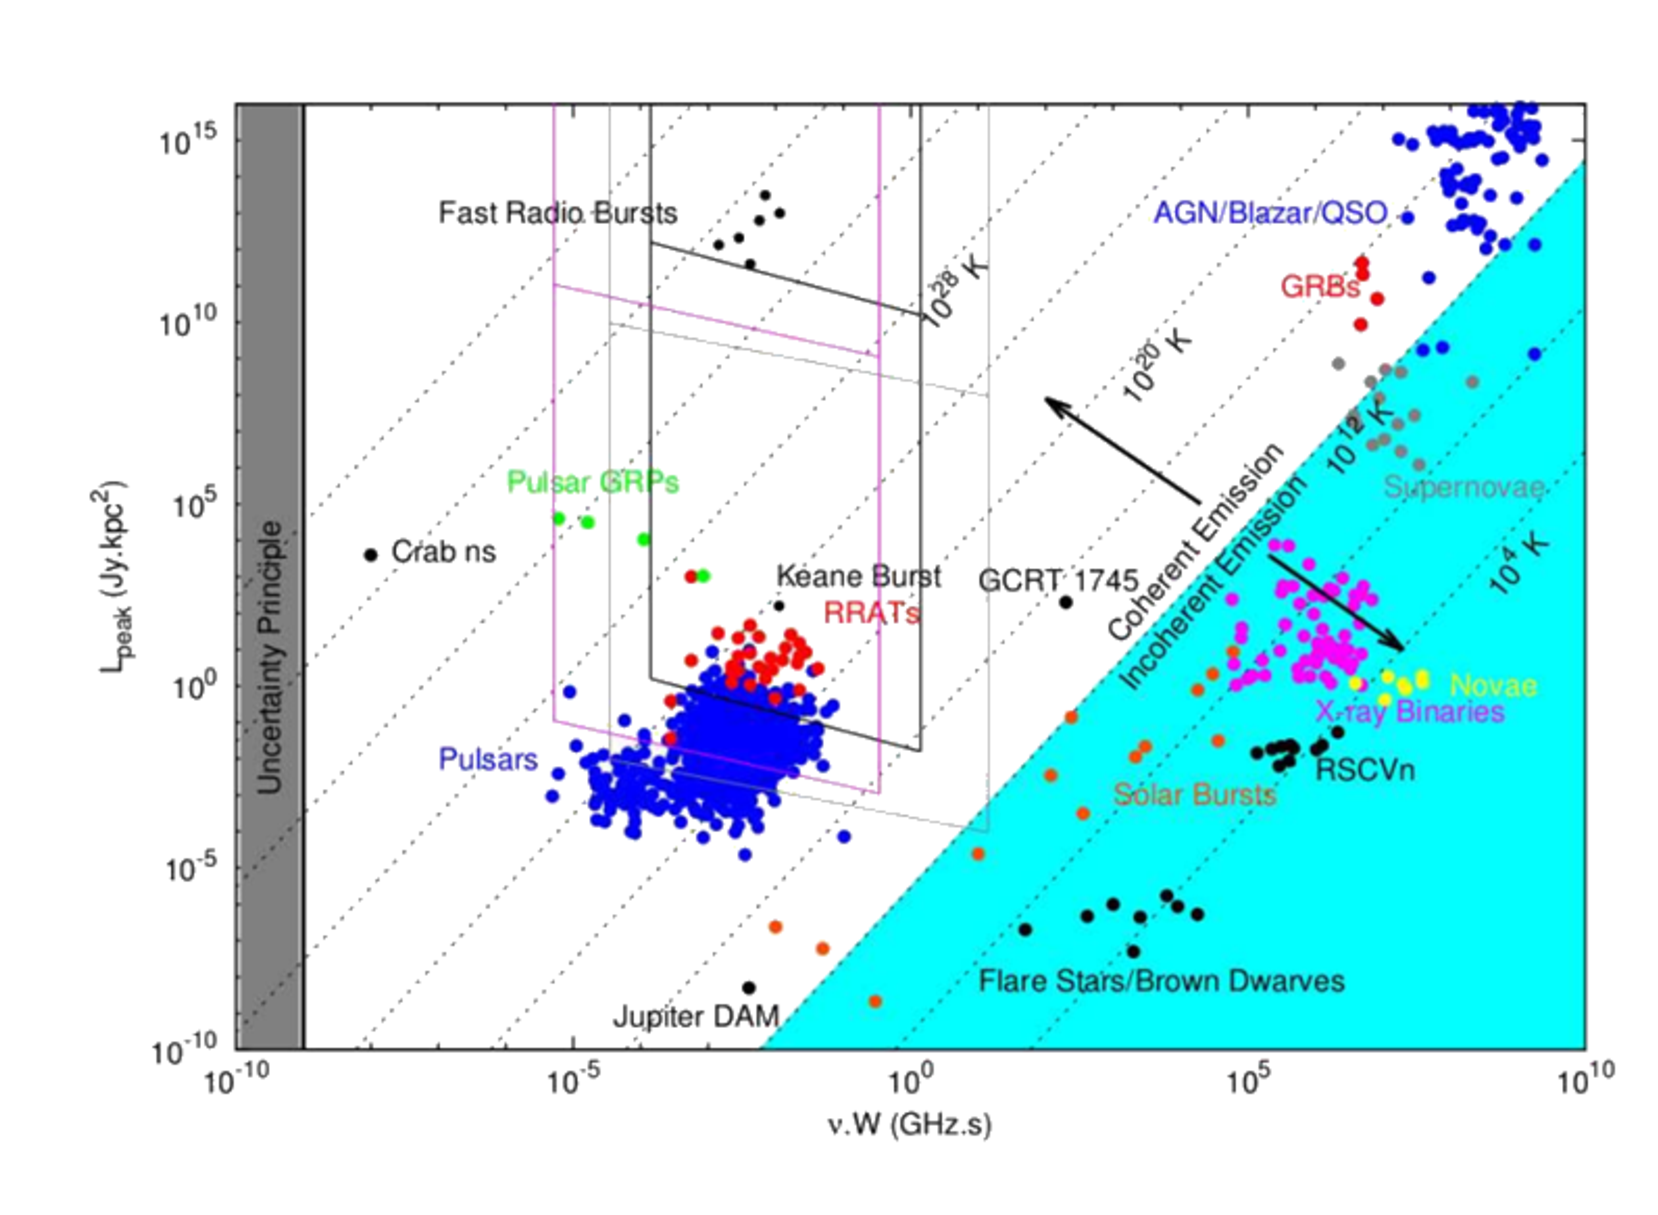
\includegraphics[width=0.9\textwidth]{transients/transients.phasespace.eps}
	\caption{突発・変動現象の相空間 (Cordes et al., in prep)。縦軸は光度変動の極大値、横軸はその変動のタイムスケールを意味し、各プロットは現象を表す。}
	\label{fig:transients.phasespace}
\end{figure}%
%コヒーレントな放射をする突発現象としては、例えばパルサーからのパルスやFRBが挙げられ、光度変動のタイムスケールは数秒以下と短い。
%変動している時間が短いため、それらは時系列の生データを解析することによって発見される。
%一方インコヒーレントな放射をする突発現象としては、例えばX線連星 (中性子星と恒星の連星など) からのバーストや超新星爆発が挙げられ、それらの多くは光度変動のタイムスケールが比較的長い。
%それらの変動は短くとも数日以上続き、たいていの場合数か月以上続くため、イメージング観測による画像データの中から発見されることが多い。

%%
\subsubsection{突発天体・変動天体の相空間}
%%
種々の突発天体をプロットした\Figref{fig:transients.phasespace}は、天体の光度$SD^2$とその変動の継続時間$W$が
\begin{align}
	SD^2 = 2 \pi k_\text{B} T (\nu W)^2, \quad \text{i.e.,} \quad
	\left( \frac{S}{\text{Jy}} \right) \left( \frac{D}{\text{kpc}} \right)^2 = 9.11 \times 10^{-18} \times
		\left( \frac{T}{\text{K}} \right) \left( \frac{\nu}{\text{GHz}} \cdot \frac{W}{\text{s}} \right)^2,
	\label{eq:transients.phasespace}
\end{align}
で関係付けられることに基づいている。
ここで$S$はフラックス密度、$D$は天体までの距離、$k_\text{B}$はボルツマン定数、$T$は輝度温度、$\nu$は観測周波数、$W$は変動の継続時間を表す。
%\footnote{電波の輝度温度とは、その電波が黒体から放射されたと見なしたときの、その黒体のもつ熱力学温度に等しい温度のこと。}
\Figref{fig:transients.phasespace}では縦軸に$SD^2~(=L_\text{peak})$、横軸に$\nu W$を取っており、複数の右上がりの直線は異なる温度$T$における\Eqref{eq:transients.phasespace}を図示したものである。

ここで\Eqref{eq:transients.phasespace}は以下のように導かれる。
レイリー・ジーンズ近似のもとで、電波天体の放射強度は $I_\nu \simeq 2\nu^2 k_\text{B} T / c^2$ と与えられる。
ここで$c$ は光速を表し、その他の量は前述のとおりである。
観測者から見た放射源の角度半径を $\theta_\text{src}$とすると、観測者の受信するフラックス密度$S$はその定義から
\begin{equation}
	S = \int_0^{2\pi} \td \phi \int_0^{\theta_\text{src}} \td \theta \sin \theta \cdot I_\nu \cos \theta
\end{equation}
で与えられる。
ここで実際の放射源の半径を $R_\text{src}$、観測者から放射源までの距離を$D$とすると、 $|\theta_\text{src}| \ll 1$であるから$\theta_\text{src} \simeq \tan \theta_\text{src} = R_\text{src} / D$と近似してよい。
また放射源の大きさ$R_\text{src}$ は変動の継続時間 $W$を用いて $R_\text{src} \simeq c W$として見積もることができるので、結局$\theta_\text{src} \simeq cW/D$と表せる。
したがってフラックス密度は
\begin{equation}
	S \simeq \pi \left( \frac{cW}{D} \right)^2 \cdot \frac{2\nu^2 k_\text{B} T}{c^2}
\end{equation}
と書け、これを変形すると\Eqref{eq:transients.phasespace}を得る。
以上のようにして、変動の継続時間 $W$ はその光度 $SD^2$ と関連付けられることがわかる。
この関係は、レイリー・ジーンズ近似、 $\theta_\text{src} \simeq \tan \theta_\text{src}$および$R_\text{src} \simeq c W$という3つの妥当な近似に基づいている。

以上のように\Figref{fig:transients.phasespace}は\Eqref{eq:transients.phasespace}に基づいた相空間を表しているが、その相空間は放射の輝度温度によって2つの領域 (白色と水色の領域) に分けられる。
地球で観測できる電波放射現象の多くは、インコヒーレントなシンクロトロン放射からなる。
しかしシンクロトロン電波の光子に電子が衝突する逆コンプトン効果によって、その光子はX線のエネルギーにまで叩き上げられ、結果的に電波の強度は制限されるという現象が起こる。
その制限された電波強度は、輝度温度にして$10^{12}~\text{K}$であり、もしある天体の輝度温度がその値を超えていた場合、その放射はコヒーレント放射かドップラー増幅されていることになる。
この輝度温度$10^{12}~\text{K}$の直線が、\Figref{fig:transients.phasespace}でコヒーレント放射の領域 (白色) とインコヒーレント放射の領域 (水色) を区切っている。

\Figref{fig:transients.phasespace}はすべての突発現象を網羅しているわけではないが、この相空間に広がる空白領域は、まだ発見されていない現象が数多く眠っていることを表している。
未知の現象があるということは、それを発見できれば新たな物理を開拓できる可能性があるということであり、科学はそのような未知の発見によって発展してきた。
したがって、\Figref{fig:transients.phasespace}の空白領域を埋めるような観測を積極的に行い、未知の現象を発見していくことが天文学者にとって重要な仕事となる。
その仕事を効率的に進めるには、高い感度と広い視野によって広範囲を探査することが必要であり、SKAはまさにそのような探査を可能とする。


\subsection{超新星} \label{transients.s1.sn}
超新星 (supernova; SN) は、星がその生涯の最期に爆発する現象であり、その爆発の実体として2つのシナリオが考えられている。
一方は、何らかの理由で白色矮星\footnote{恒星の場合、気体の圧力や核融合による輻射圧が重力とつりあって形状を保っており、白色矮星の場合は電子の縮退圧、中性子星の場合は中性子の縮退圧が、重力とつりあっている。}の質量が増大しチャンドラセカール質量\footnote{重力が電子の縮退圧を超える限界質量をチャンドラセカール質量とよび、それを超えた白色矮星は超新星爆発を起こす。}に達した時に、核暴走により白色矮星自体が爆発するというものである。
白色矮星質量を増大させる機構として、白色矮星と恒星の連星系において恒星のガスが白色矮星に降着するシナリオ、二つの白色矮星が重力波
放出を通し合体するシナリオが提案されている。
同様に白色矮星を起源とした核暴走として新星爆発が知られているが、この二つではその爆発の規模が大きく異なる。
新星爆発の場合は、白色矮星の表面上で一時的に核融合が暴走し爆発するだけで、白色矮星自体は爆発後も健在だが、超新星爆発の場合は白色矮星全体が爆発してしまい、後には何も残らず四散してしまうと考えられている。
もう一方のシナリオは、大質量星が自重を支えきれずに単独で重力崩壊し爆発するというものである。
大質量の恒星は内部に鉄などのコアをもつが、そのコアが重力崩壊を起こすと中心部に硬い原始中性子星がつくられ、それに衝突した物質がはね返って衝撃波をつくり爆発すると考えられている。% \citep[e.g.,][]{1994Natur.371..227N}。
このシナリオの超新星は、コアが重力崩壊することにちなんで、コア崩壊型超新星 (core-collapse supernova; CCSN) または重力崩壊型超新星とよばれる。
これらのシナリオは妥当なものだが、爆発に至る詳しいメカニズムはわかっておらず、コンピュータシミュレーションや観測事実の蓄積によって、その解明が試みられている。
超新星の分類は、歴史的にはスペクトルや光度曲線の特性によって行われ、\Figref{fig:transients.s1.sn}のように分類され命名されてきている。
連星系にある白色矮星の超新星爆発はIa型超新星に分類され、その他のIb型、Ic型、II型超新星はすべてコア崩壊型超新星である。
%例えばスペクトルに水素の吸収線が見られるものはII型に分類されるが、吸収線があるということは水素が豊富であることを示しており、\Figref{fig:transients.s1.sn}の右図のように水素が多く含まれた星が爆発したものと考えられる。
\begin{figure}[]
	\begin{minipage}{0.6\textwidth}
		\centering
		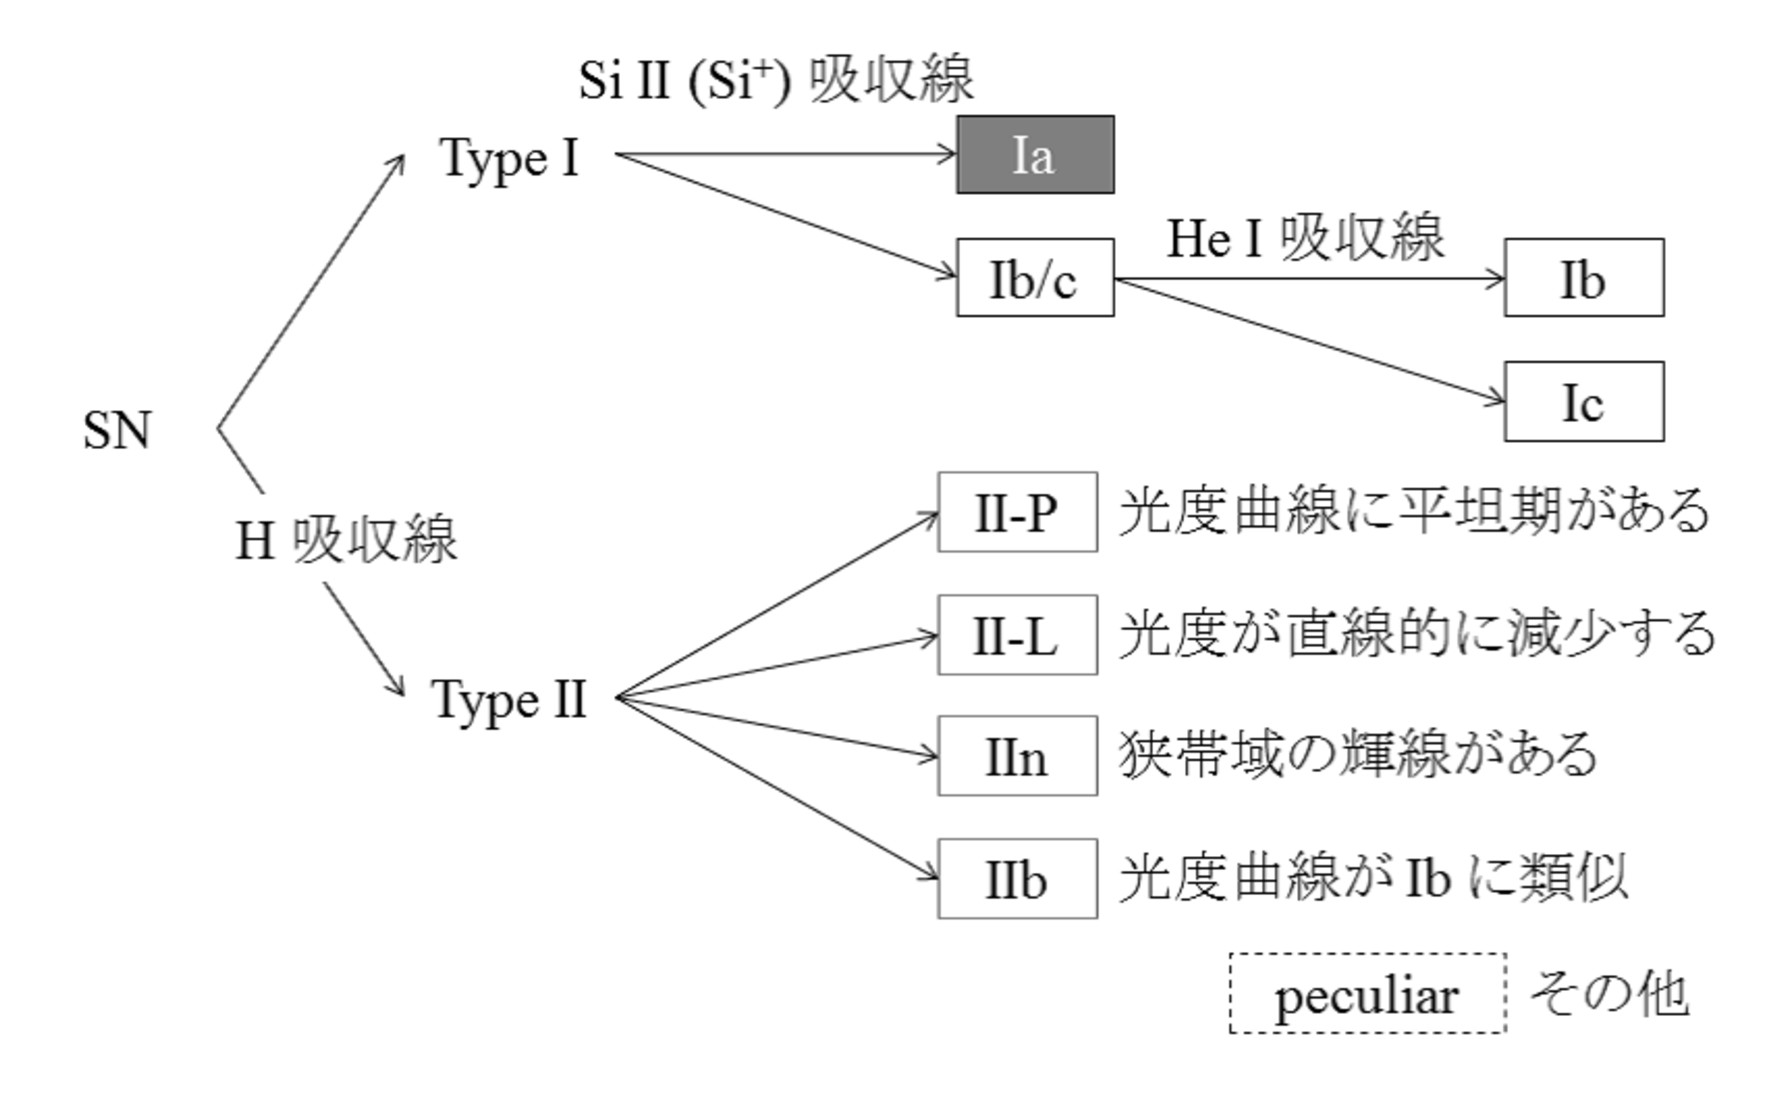
\includegraphics[width=\linewidth,clip]{transients/transients.s1.sn-class.eps}
	\end{minipage}
	\begin{minipage}{0.4\textwidth}
		\centering
		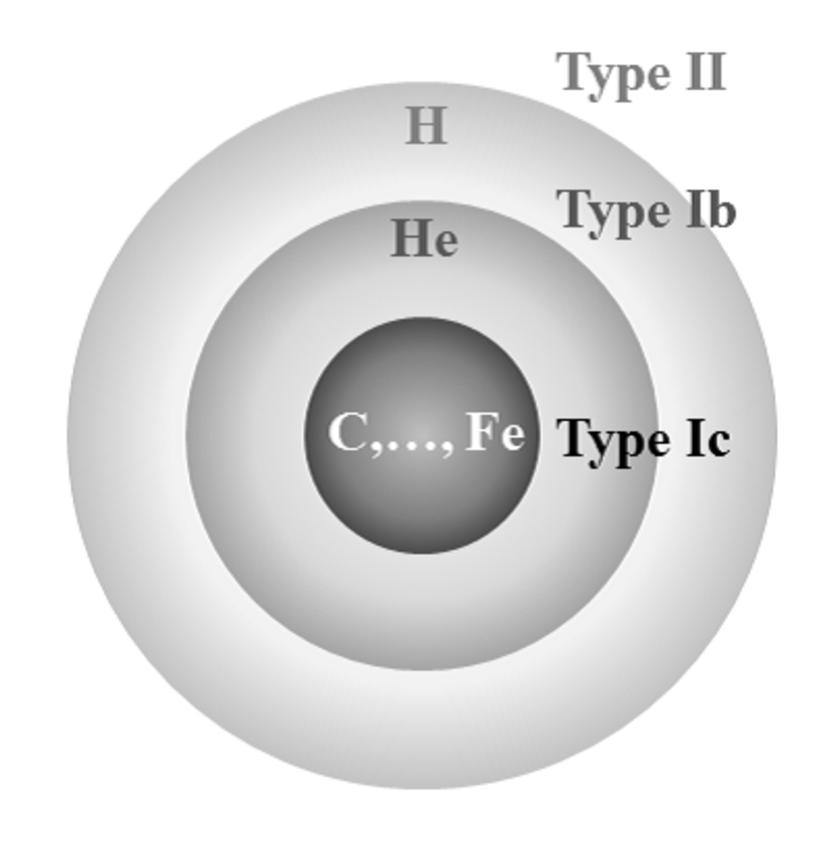
\includegraphics[width=0.7\linewidth,clip]{transients/transients.s1.ccsn.eps}
	\end{minipage}
	\caption{左図: 超新星の分類; 右図: コア崩壊型超新星となる以前の星の「たまねぎ構造」。}
	\label{fig:transients.s1.sn}
\end{figure}%

超新星爆発は主に光学望遠鏡によって発見され、電波望遠鏡で先んじて発見されたことはほとんどなかった。
%これは可視光域で明るいという理由の他に、光学望遠鏡は広い範囲を高い空間分解能で観測することに長けており、突発天体を発見しやすい装置であることも一因として挙げられる。
%またその探査では日本のアマチュア天文家による貢献も大きい。
%一方で従来の電波望遠鏡は、狭い範囲を極めて高い空間分解能で観測することに長けており\footnote{電波望遠鏡は、広い範囲を低い空間分解能で観測することにも長けている。}、それゆえ光学望遠鏡で発見された超新星を詳細に追観測することが主な役割だった。
SKAではこの状況を打破し、光学望遠鏡で発見された超新星の追観測のみならず、広い視野による広域探査によって電波帯域における超新星の発見を目指す。
また従来、Ia型超新星は暗すぎるために電波で検出されたことがないが \citep{2012ApJ...750..164C}、SKAによって初めてIa型超新星の電波観測が成功すると期待される。

超新星からの電波は、爆発の瞬間に放射されるのではなく、爆発前に星から噴出した物質に対して、爆発後に噴出した物質が衝突することによって放射されると考えられている。
したがって超新星を電波観測すると、爆発前後の星の状態を調べることができる。
また減光した後も、その噴出物は周りの星間物質と相互作用し続け、超新星残骸 (supernova remnant; SNR) とよばれる構造をなす。
その中では宇宙線の起源となる粒子加速が起こっていると考えられ、超新星残骸の電波観測によって他波長にわたる物理過程の解明が進むだろう。
可視光域で発見されている超新星のうち、従来の電波望遠鏡で観測できているものは一握りであるため、SKAによる高感度観測によって電波による観測サンプル数が増えれば、超新星の研究にとって大きなブレイクスルーとなるに違いない。

%%
%% GRB
%%
\subsection{ガンマ線バースト} \label{transients.s1.grb}
ガンマ線バースト (gamma-ray burst; GRB) は極めて遠方の銀河における突発的なガンマ線放射現象であり、その放射の継続時間によって2種類に分類され、継続時間が数秒以上と長いものを long-duration GRB、それ以下のものを short-duration GRB とよぶ。
GRBの大半は long GRB が占めており、他波長域でとても明るい残光が観測され、その実体は大質量星が重力崩壊したときの超新星爆発だと考えられている \citep{2006ARA&A..44..507W}。
またそのほとんどが星形成の盛んな銀河で発見される。
一方で short GRB は、中性子星やブラックホールなどの連星合体による爆発だと考えられ、星形成が活発ではない銀河で発見されている \citep{2007PhR...442..166N}。
連星合体は重力波源としてもっとも有力な候補でもあり、また\Secref{transients.s1.frb}で述べるFRBとの関連性も指摘されている \citep{2013PASJ...65L..12T}。

%%
%% Afterglow
%%
\subsubsection{GRB Afterglows}
GRBに伴う残光 (afterglow) は、ガンマ線が放射されてしばらく経ってから他波長域で明るく輝きだす現象である。
これは天体からジェットとして放出された物質が、星間物質に衝突することによって電磁波が放射されるというファイアーボールモデルでおおよそ説明でき \citep{1999PhR...314..575P}、GRB発生から残光として輝きだすまでの時間は場合によって異なる。
このGRB残光の光度曲線やスペクトル特性などから、GRBの発生機構や母銀河の構成成分などを知ることができ、そのためにはGRBの発生直後から他波長で継続して追観測することが重要となる。

それを実現するための追観測体制は世界的に整えられてきており\footnote{GRBの発見速報システムとしてNASAによるGRB Coordinates Network (GCN) があり、GRB発見後2秒以内にその位置情報などを他観測局へ速報し、迅速な追観測が可能になっている。}、ガンマ線観測衛星の発見速報を受けた他の観測局が、他波長でそれを詳細に追観測することが可能となっている。
それによってGRBの研究は最近10年程度で大きく前進し、超新星との関連性などいろいろな情報が得られ、先に述べたような実体の解明が進んでいる。
高感度なSKAでは、従来の望遠鏡では観測できなかった暗い電波残光をも観測できるため、この研究をさらに前進させGRBの統一描像の構築や、宇宙初期の様相の解明に大きく貢献するだろう。

%%
%% Orphan Afterglow
%%
\subsubsection{Orphan GRB Afterglows}
\begin{wraptable}{r}{2.5cm}
	\vspace{-4zh}
	\hspace{-4zw}
	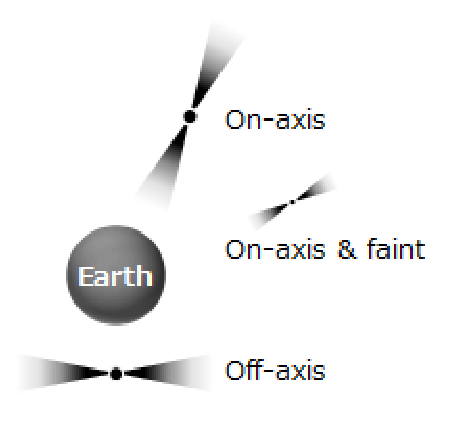
\includegraphics[width=3.5cm,clip]{transients/transients.GRB-afterglow.eps}
\end{wraptable}
GRBのガンマ線放射は高い指向性があり、その軸方向のみにガンマ線を放射するため、放射軸上に地球がなければガンマ線は観測されない。
一方でそれに付随する残光は指向性が高くないため、地球では残光のみが観測される、という状況を考えることができる \citep{1997ApJ...487L...1R}。
このような残光は親なし残光 (orphan afterglow) と呼ばれ、対応天体の見つからない電波トランジェントとして観測されうる\footnote{ガンマ線放射の軸が地球に向いていることを on-axis、向いていないことを off-axis と呼び、orphan afterglow は off-axis GRB afterglow と言い換えることができる。}。
\citet{2001ApJ...562L..55F}の見積もりによれば、99\% 以上のGRBで放射軸が地球から外れておりorphan afterglow のみが観測されると考えられるものの、従来の観測では候補天体が数例報告されているだけで、確定には至っていない。
SKAの広視野・高感度サーベイによって orphan afterglow を発見することができれば、GRB の物理の解明は大きく前進すると期待できる。
%

%

\subsection{ブラックホールによる星の潮汐崩壊} \label{transients.s1.tde}
超巨大ブラックホール (supermassive black hole; SMBH) のまわりを回る星々は、そのブラックホールから強い潮汐力を受け、もしその潮汐力の大きさが星の重力を越えると、その星は形状を保つことができず崩壊してしまう。
これを潮汐崩壊現象 (tidal disruption event; TDE) とよび、その際、まれにジェットを伴う爆発を起こし急激に光度を増す。

そのようなジェットを伴う潮汐崩壊現象は、特異的なガンマ線バーストとしてSwift衛星によって初めて観測され Swift J1644+57 (GRB 110328A) と命名された。
発見当初は起源がわからなかったが、その後、X線、赤外線、電波の追観測によって残光が観測され \citep{2011Sci...333..199L}、潮汐崩壊現象と考えられるにいたった \citep{2011Sci...333..203B}。
SKAはこの潮汐崩壊現象を数多く発見できると考えられ、銀河中心ブラックホールの物理に迫ることができるだろう。


%%\subsection{Magnetars (Anomalous X-ray Pulsars, Soft Gamma Repeaters)} \label{transients.s1.magnetars}

\subsection{Fast Radio Bursts (FRBs)} \label{transients.s1.frb}
銀河系外からの電波パルスは、1930年代に電波天文学が拓かれて以降近年に至るまで、発見されてこなかった。
つまり\Tabref{tb:frail-classification}の左上の欄は、近年まで空白のままであった。
しかしついに2007年、銀河系外起源と思われる電波パルスがオーストラリアParkes 64~m 電波望遠鏡によって発見された \citep{2007Sci...318..777L}。
そのパルスは幅数ミリ秒と短寿命かつ大強度であり、さらに発見された位置が高銀緯にも関わらず分散測度 (dispersion measure; DM) が極めて大きいことから、その起源は銀河系外の高エネルギー天体だと考えられた\footnote{
最初に発見されたFRB~010724 (Lorimer burst) は、パルス幅が $W=5~\text{ms}$、フラックス密度が $S_{1.4~\text{GHz}}=30~\text{Jy}$、また発見された位置が銀緯$b = -41.8\arcdeg$、パルスの分散測度は$\text{DM} \sim 375~\text{pc}~\text{cm}^{-3}$であった。
それから推定される地球からの距離はおよそ500~Mpcと考えられ、また遠くとも1~Gpc以内の天体だと考えられている。
}。
さらにパルス放射はその1発限りであり、それ以降同じ場所からの電波放射は確認されていない。

このような現象は従来報告されておらずその信憑性が疑われたこともあり、しばらくは発見者の名前をとってLorimer burst と呼ばれていたが、同様のパルスが \citet{2011MNRAS.415.3065K} および \citet{2013Sci...341...53T} によって新たに5例発見され、この銀河系外からの電波パルスは fast radio bursts (FRBs) と呼ばれるに至った。
このFRBの起源はわかっておらず、そもそもPerytonと命名されている地球起源の謎のノイズ \citep{2011ApJ...727...18B} との区別も明確ではない。
しかしその後、オーストラリアから遠く離れたプエルトリコのArecibo 300~m 電波望遠鏡によって同様のFRBが1例発見され \citep{2014ApJ...790..101S}、FRBが宇宙起源の天体現象であることの信頼性は非常に高まっている。
起源天体のモデルとしては多くの説が唱えられており、
銀河系内からの放射では説明しにくいことが様々な研究で示されている \citep[e.g.,][]{2014ApJ...797...70K}。
%ただし一方で系内起源を主張する研究もあり \citep[e.g.,][]{2014MNRAS.439L..46L}。
%例えば中性子星連星の合体に伴う電波放射モデルが提案されており (\citealt{2013PASJ...65L..12T})、合体に伴う重力波放射との一致性が確認されれば宇宙物理学に大きな影響を与えるだろう。


%%
%% Unknowns
%%
\subsection{未知の突発天体} \label{transients.s1.unknowns}
本節では電波帯域でのみ観測され、他の波長帯域やあるいは電波帯域ですら対応天体が見つかっていないような未知の突発天体について紹介する。
併せて、既知の天体と同定はできているものの、その放射過程が未解明な天体についても述べる。
その紹介にあたっては観測方法に着目した\Tabref{tb:frail-classification}の分類法に従い、その天体が銀河系外か系内にあるか、短時間変動か長時間変動か、という4種類に分けて述べる。

%%
%% ss1
%%
\subsubsection{種類1: 銀河系内の短時間変動天体}
銀河系内の天体に起源を持ち、変動の継続時間が数秒以下のパルスを発する天体として代表的なものはパルサー、つまり自転する中性子星である。
それらパルサーの中でも、Crab nanoshots や RRATs といった特殊なパルス放射現象が報告されおり (次項参照)、それらの現象は突発天体研究においても興味深い研究対象である。
また銀河系内でパルス状の電波放射をする天体としては中性子星のみが知られており、それ以外の系内天体で電波パルスは観測されていないが、今後、中性子星起源とは考えられないような電波パルスが観測されることもあるかもしれない。
そのような未知の突発現象観測には、従来の望遠鏡を越える感度と高い時間分解能、そしてデータ解析コンピュータの計算速度が要求される。

%%
\paragraph{Crab Nanoshots}
電波パルサーの中には、通常のパルス放射とは異なる放射をするパルサーがあることが、近年明らかになってきている。
Crabパルサーから放たれるパルスは、そのパルス幅が 3~ms、パルス周期が 33~msであり、そのフラックス密度は平均して 14~mJyである。
一方で時折、大強度のジャイアントパルスを放つことがあり、そのフラックス密度は 1~MJy に達することもある。
このジャイアントパルスの中で、パルス幅が通常よりも極端に短くなる現象がArecibo 電波望遠鏡を用いた周波数 9.25~GHz の観測によって明らかとなった。
そのパルス幅は観測の時間分解能 0.4~ns より短く、フラックス密度は 2~MJy という極めて短寿命で大強度のパルスであり、nanoshots と呼ばれた \citep{2003Natur.422..141H,2007ApJ...670..693H}。
そのパルスの放射源の大きさは 12~cm、輝度温度は$10^{41}~\text{K}$と見積もられ、高エネルギーかつコンパクトな天体現象である。

発見者らはこのnanoshotsを説明できる唯一のモデルとして \citet{1998ApJ...506..341W} によって提示されたプラズマ乱流モデルを挙げているが、その放射機構は必ずしも解明されていない。
また同様にパルス幅が短くなる現象は他のパルサーでは確認されておらず、現状ではCrabパルサーに特有の現象である。
さらにはジャイアントパルスでのみ起こるのか、本質的には通常のパルスでも起こっているが感度不足で検出できていないだけなのかという点もわかっていない。
SKAを用いた高感度観測によってnanoshotsについてより詳しい知見が得られれば、パルサー磁気圏の研究が大きく進むと期待できる。

%%
\paragraph{RRATs}
通常のパルサーとは異なるパルス放射天体としては、Parkes 64~m 電波望遠鏡で発見された rotating radio transients (RRATs) が挙げられる \citep{2006Natur.439..817M}。
このRRATsはパルサーと同様に強い磁場を持つ中性子星が起源だと考えられているが、パルサーの周期的なパルス放射とは異なり、その放射は散発的で放射機構は明らかとなっていない。
SKAを用いてRRATsを高感度で観測すれば、その散発性についてより詳しい議論が可能になるだろう。


%%
%% ss2
%%
\subsubsection{種類2: 銀河系外の短時間変動天体}
銀河系外からの電波パルスは、\Secref{transients.s1.frb}で述べたFRBのみである\footnote{FRBは\Secref{transients.s1.frb}で述べたように銀河系内を起源とする説もあり、必ずしも系外天体として見解が一致しているわけではない。}。
FRBは従来予想もされていなかった現象であり、発見当初はそれほど大きな注目を集めていなかった。
しかしその後アーカイブデータの解析によって続々と発見されたため、現在は大きな注目を集め、SKAによる重要なサイエンスの一部を担うに至っている。
FRBのような未知の天体は、まだ宇宙に多く眠っていると考えられ、それらを発見するには柔軟な観測システムが必要となり、SKAはそれを実装しなければならない (\Secref{transients.s2.fender})。

%%
%% ss3
%%
\subsubsection{種類3: 銀河系内の長時間変動天体}
銀河系内を起源とした数秒以上の長時間変動を示す天体は数多くあり、例えば\Tabref{tb:frail-classification}に挙げた恒星フレアやメーザーバースト、X線連星における電波バーストなど多種多様である。
それらのほとんどは対応天体が見つかりやすく、起源がわかっているものが多い。

一方で対応天体が同定されていないものもあり、例えば\citet{2005Natur.434...50H} が銀河中心近傍に発見した周期的なバースト現象が挙げられる。
このバーストはフラックス密度が 1~Jy、1回のバーストの幅が 10 分でそのバーストが 77 分周期に5回現れるという特異的な突発現象であり、VLA を用いた観測によって発見された。
この天体は GCRT J1745-3009 と名付けられ\footnote{接頭辞 GCRT は Galactic Center Radio Transient の頭文字をとったものである。}、対応天体は見つかっておらず放射機構も不明である。
しかしその後の追観測によって同じ場所から同様のバーストが観測され、\citet{2010ApJ...712L...5R} によって偏波情報が明らかとなった。

その情報などから起源についていくつかのモデルが発案されており、その中には、一時的にパルス放射が消える nulling pulsar (\citealp{2005Natur.434...28K})、中性子星連星 (\citealp{2005ApJ...628L..49T})、白色矮星 (\citealp{2005ApJ...631L.143Z})、歳差運動するパルサー (\citealp{2006MNRAS.365L..16Z})、恒星フレア (\citealp{2010ApJ...712L...5R}) などがある。
以上のように起源について多くのモデルは考えられているが、それらについて確証は得られていない。
このような数分スケールのバースト現象の探査は大規模には行われておらず、SKAにおいてもデータ解析システムに対して同様のバーストを効率的に探査する機能を要求する必要がある。

%%
%% ss4
%%
\subsubsection{種類4: 銀河系外の長時間変動天体}
銀河系外における長時間変動を示す天体のうち、対応天体が見つかりにくく未知天体と認識されるものとして代表的なのは、orphan GRB afterglow (\Secref{transients.s1.grb}) や TDE (\Secref{transients.s1.tde}) であろう。
GRB残光や超新星爆発に代表される突発現象は、電波帯域では増光は急激だが減光は緩やかで、その継続時間は数か月以上に及ぶものも多い。
一方、変動の継続時間が数か月以下で、起源が未知の突発天体がいくつか報告されている。

例えばVLA のアーカイブデータからは4つの候補天体が発見されており、特にRT~19920826と命名されたものについては検出状態も良好であった \citep{2007ApJ...666..346B,2012ApJ...747...70F}。%
同様の突発天体は早稲田大学の那須パルサー観測所においても発見され、WJN~J1443+3439と命名された天体があるが、その起源については恒星フレアやAGNフレアが示唆されているものの、必ずしもわかっていない \citep{2007ApJ...657L..37N,2014ApJ...781...10A}。
そのような未知の突発天体を探査し、\Figref{fig:transients.phasespace}の空白領域を埋めるには、広い視野を高感度で探査し、さらに様々な時間分解能でデータ処理するための解析システムが必要になる。

%%\subsubsection{LOFAR Transients を加筆}

